% Options for packages loaded elsewhere
\PassOptionsToPackage{unicode}{hyperref}
\PassOptionsToPackage{hyphens}{url}
\PassOptionsToPackage{dvipsnames,svgnames,x11names}{xcolor}
%
\documentclass[
  a4paper,
]{article}
\usepackage{amsmath,amssymb}
\usepackage{iftex}
\ifPDFTeX
  \usepackage[T1]{fontenc}
  \usepackage[utf8]{inputenc}
  \usepackage{textcomp} % provide euro and other symbols
\else % if luatex or xetex
  \usepackage{unicode-math} % this also loads fontspec
  \defaultfontfeatures{Scale=MatchLowercase}
  \defaultfontfeatures[\rmfamily]{Ligatures=TeX,Scale=1}
\fi
\usepackage{lmodern}
\ifPDFTeX\else
  % xetex/luatex font selection
\fi
% Use upquote if available, for straight quotes in verbatim environments
\IfFileExists{upquote.sty}{\usepackage{upquote}}{}
\IfFileExists{microtype.sty}{% use microtype if available
  \usepackage[]{microtype}
  \UseMicrotypeSet[protrusion]{basicmath} % disable protrusion for tt fonts
}{}
\makeatletter
\@ifundefined{KOMAClassName}{% if non-KOMA class
  \IfFileExists{parskip.sty}{%
    \usepackage{parskip}
  }{% else
    \setlength{\parindent}{0pt}
    \setlength{\parskip}{6pt plus 2pt minus 1pt}}
}{% if KOMA class
  \KOMAoptions{parskip=half}}
\makeatother
\usepackage{xcolor}
\usepackage[margin = 2cm]{geometry}
\usepackage{color}
\usepackage{fancyvrb}
\newcommand{\VerbBar}{|}
\newcommand{\VERB}{\Verb[commandchars=\\\{\}]}
\DefineVerbatimEnvironment{Highlighting}{Verbatim}{commandchars=\\\{\}}
% Add ',fontsize=\small' for more characters per line
\usepackage{framed}
\definecolor{shadecolor}{RGB}{248,248,248}
\newenvironment{Shaded}{\begin{snugshade}}{\end{snugshade}}
\newcommand{\AlertTok}[1]{\textcolor[rgb]{0.94,0.16,0.16}{#1}}
\newcommand{\AnnotationTok}[1]{\textcolor[rgb]{0.56,0.35,0.01}{\textbf{\textit{#1}}}}
\newcommand{\AttributeTok}[1]{\textcolor[rgb]{0.13,0.29,0.53}{#1}}
\newcommand{\BaseNTok}[1]{\textcolor[rgb]{0.00,0.00,0.81}{#1}}
\newcommand{\BuiltInTok}[1]{#1}
\newcommand{\CharTok}[1]{\textcolor[rgb]{0.31,0.60,0.02}{#1}}
\newcommand{\CommentTok}[1]{\textcolor[rgb]{0.56,0.35,0.01}{\textit{#1}}}
\newcommand{\CommentVarTok}[1]{\textcolor[rgb]{0.56,0.35,0.01}{\textbf{\textit{#1}}}}
\newcommand{\ConstantTok}[1]{\textcolor[rgb]{0.56,0.35,0.01}{#1}}
\newcommand{\ControlFlowTok}[1]{\textcolor[rgb]{0.13,0.29,0.53}{\textbf{#1}}}
\newcommand{\DataTypeTok}[1]{\textcolor[rgb]{0.13,0.29,0.53}{#1}}
\newcommand{\DecValTok}[1]{\textcolor[rgb]{0.00,0.00,0.81}{#1}}
\newcommand{\DocumentationTok}[1]{\textcolor[rgb]{0.56,0.35,0.01}{\textbf{\textit{#1}}}}
\newcommand{\ErrorTok}[1]{\textcolor[rgb]{0.64,0.00,0.00}{\textbf{#1}}}
\newcommand{\ExtensionTok}[1]{#1}
\newcommand{\FloatTok}[1]{\textcolor[rgb]{0.00,0.00,0.81}{#1}}
\newcommand{\FunctionTok}[1]{\textcolor[rgb]{0.13,0.29,0.53}{\textbf{#1}}}
\newcommand{\ImportTok}[1]{#1}
\newcommand{\InformationTok}[1]{\textcolor[rgb]{0.56,0.35,0.01}{\textbf{\textit{#1}}}}
\newcommand{\KeywordTok}[1]{\textcolor[rgb]{0.13,0.29,0.53}{\textbf{#1}}}
\newcommand{\NormalTok}[1]{#1}
\newcommand{\OperatorTok}[1]{\textcolor[rgb]{0.81,0.36,0.00}{\textbf{#1}}}
\newcommand{\OtherTok}[1]{\textcolor[rgb]{0.56,0.35,0.01}{#1}}
\newcommand{\PreprocessorTok}[1]{\textcolor[rgb]{0.56,0.35,0.01}{\textit{#1}}}
\newcommand{\RegionMarkerTok}[1]{#1}
\newcommand{\SpecialCharTok}[1]{\textcolor[rgb]{0.81,0.36,0.00}{\textbf{#1}}}
\newcommand{\SpecialStringTok}[1]{\textcolor[rgb]{0.31,0.60,0.02}{#1}}
\newcommand{\StringTok}[1]{\textcolor[rgb]{0.31,0.60,0.02}{#1}}
\newcommand{\VariableTok}[1]{\textcolor[rgb]{0.00,0.00,0.00}{#1}}
\newcommand{\VerbatimStringTok}[1]{\textcolor[rgb]{0.31,0.60,0.02}{#1}}
\newcommand{\WarningTok}[1]{\textcolor[rgb]{0.56,0.35,0.01}{\textbf{\textit{#1}}}}
\usepackage{longtable,booktabs,array}
\usepackage{calc} % for calculating minipage widths
% Correct order of tables after \paragraph or \subparagraph
\usepackage{etoolbox}
\makeatletter
\patchcmd\longtable{\par}{\if@noskipsec\mbox{}\fi\par}{}{}
\makeatother
% Allow footnotes in longtable head/foot
\IfFileExists{footnotehyper.sty}{\usepackage{footnotehyper}}{\usepackage{footnote}}
\makesavenoteenv{longtable}
\usepackage{graphicx}
\makeatletter
\def\maxwidth{\ifdim\Gin@nat@width>\linewidth\linewidth\else\Gin@nat@width\fi}
\def\maxheight{\ifdim\Gin@nat@height>\textheight\textheight\else\Gin@nat@height\fi}
\makeatother
% Scale images if necessary, so that they will not overflow the page
% margins by default, and it is still possible to overwrite the defaults
% using explicit options in \includegraphics[width, height, ...]{}
\setkeys{Gin}{width=\maxwidth,height=\maxheight,keepaspectratio}
% Set default figure placement to htbp
\makeatletter
\def\fps@figure{htbp}
\makeatother
\setlength{\emergencystretch}{3em} % prevent overfull lines
\providecommand{\tightlist}{%
  \setlength{\itemsep}{0pt}\setlength{\parskip}{0pt}}
\setcounter{secnumdepth}{-\maxdimen} % remove section numbering
\usepackage{fvextra}
\DefineVerbatimEnvironment{Highlighting}{Verbatim}{breaklines,breaksymbolleft={},commandchars=\\\{\}}
\usepackage{tcolorbox}
\usepackage{graphicx}
\usepackage{booktabs}
\usepackage[default]{lato}
\usepackage{bm}
\usepackage{ulem}
\ifLuaTeX
  \usepackage{selnolig}  % disable illegal ligatures
\fi
\usepackage[style=apa,]{biblatex}
\addbibresource{references.bib}
\IfFileExists{bookmark.sty}{\usepackage{bookmark}}{\usepackage{hyperref}}
\IfFileExists{xurl.sty}{\usepackage{xurl}}{} % add URL line breaks if available
\urlstyle{same}
\hypersetup{
  pdftitle={Spatial Economics -- Assignment 3},
  pdfauthor={Elia Di Gregorio (h12039313@s.wu.ac.at); Max Heinze (h11742049@s.wu.ac.at); Sophia Ludescher (h11801892@s.wu.ac.at)},
  colorlinks=true,
  linkcolor={Maroon},
  filecolor={Maroon},
  citecolor={DarkOrchid!65!black},
  urlcolor={DarkOrchid!65!black},
  pdfcreator={LaTeX via pandoc}}

\title{\textbf{Spatial Economics -- Assignment 3}}
\author{Elia Di Gregorio
(\href{mailto:h12039313@s.wu.ac.at}{\nolinkurl{h12039313@s.wu.ac.at}}) \and Max
Heinze
(\href{mailto:h11742049@s.wu.ac.at}{\nolinkurl{h11742049@s.wu.ac.at}}) \and Sophia
Ludescher
(\href{mailto:h11801892@s.wu.ac.at}{\nolinkurl{h11801892@s.wu.ac.at}})}
\date{May 3, 2024}

\begin{document}
\maketitle

{
\hypersetup{linkcolor=}
\setcounter{tocdepth}{2}
\tableofcontents
}
\vspace{2em}

\begin{tcolorbox}
\centering \itshape The executable code that was used in compiling the assignment is available on GitHub at \url{https://github.com/maxmheinze/spatial}.
\end{tcolorbox}

\newpage

\hypertarget{task-a}{%
\section{Task A}\label{task-a}}

\hypertarget{nauxefve-panel-model-and-specification-search}{%
\subsection{Naïve Panel Model and Specification
Search}\label{nauxefve-panel-model-and-specification-search}}

We begin by fitting the spatially naïve panel model using the
\texttt{plm} function. The output is printed below.

\begin{Shaded}
\begin{Highlighting}[]
\NormalTok{cm1 }\OtherTok{\textless{}{-}} \FunctionTok{plm}\NormalTok{(logc }\SpecialCharTok{\textasciitilde{}}\NormalTok{ logp }\SpecialCharTok{+}\NormalTok{ logy, }\AttributeTok{data =}\NormalTok{ cigs, }\AttributeTok{effect =} \StringTok{"twoway"}\NormalTok{, }\AttributeTok{model =} \StringTok{"within"}\NormalTok{,}
    \AttributeTok{index =} \FunctionTok{c}\NormalTok{(}\StringTok{"state"}\NormalTok{, }\StringTok{"year"}\NormalTok{))}
\end{Highlighting}
\end{Shaded}

\begin{center}
\begin{tabular}{@{\extracolsep{5pt}}lc} 
\\[-1.8ex]\hline 
\hline \\[-1.8ex] 
 & \multicolumn{1}{c}{\textit{Dependent variable:}} \\ 
\cline{2-2} 
\\[-1.8ex] & logc \\ 
\hline \\[-1.8ex] 
 logp & $-$1.035$^{***}$ \\ 
  & (0.042) \\ 
  & \\ 
 logy & 0.529$^{***}$ \\ 
  & (0.047) \\ 
  & \\ 
\hline \\[-1.8ex] 
Observations & 1,380 \\ 
R$^{2}$ & 0.394 \\ 
Adjusted R$^{2}$ & 0.359 \\ 
F Statistic & 424.344$^{***}$ (df = 2; 1303) \\ 
\hline 
\hline \\[-1.8ex] 
\textit{Note:}  & \multicolumn{1}{r}{$^{*}$p$<$0.1; $^{**}$p$<$0.05; $^{***}$p$<$0.01} \\ 
\end{tabular} 
\end{center}

As the true spatial econometricians we are, we now ignore everything
that is reminiscent of economic theory and venture on a standard
specification testing path. We begin by performing a Lagrange Multiplier
test for spatial lags in both the error and the dependent. The results
are printed below.

\begin{Shaded}
\begin{Highlighting}[]
\FunctionTok{slmtest}\NormalTok{(cm1, cigm, }\AttributeTok{test =} \StringTok{"lme"}\NormalTok{)}
\end{Highlighting}
\end{Shaded}

\begin{verbatim}
## 
##  LM test for spatial error dependence
## 
## data:  formula (within transformation)
## LM = 54.655, df = 1, p-value = 1.437e-13
## alternative hypothesis: spatial error dependence
\end{verbatim}

\begin{Shaded}
\begin{Highlighting}[]
\FunctionTok{slmtest}\NormalTok{(cm1, cigm, }\AttributeTok{test =} \StringTok{"lml"}\NormalTok{)}
\end{Highlighting}
\end{Shaded}

\begin{verbatim}
## 
##  LM test for spatial lag dependence
## 
## data:  formula (within transformation)
## LM = 46.901, df = 1, p-value = 7.468e-12
## alternative hypothesis: spatial lag dependence
\end{verbatim}

As we can see, both tests return significant \(p\)-values, meaning that
we reject the null hypotheses of spatial dependence being present in the
errors or the dependent, respectively. We thus continue by performing
robust LM tests for spatial dependence in both the errors and the
dependent which account for the respectively other type of spatial
dependence potentially being present. The results of these two tests are
printed below.

\begin{Shaded}
\begin{Highlighting}[]
\FunctionTok{slmtest}\NormalTok{(cm1, cigm, }\AttributeTok{test =} \StringTok{"rlme"}\NormalTok{)}
\end{Highlighting}
\end{Shaded}

\begin{verbatim}
## 
##  Locally robust LM test for spatial error dependence sub spatial lag
## 
## data:  formula (within transformation)
## LM = 8.9106, df = 1, p-value = 0.002835
## alternative hypothesis: spatial error dependence
\end{verbatim}

\begin{Shaded}
\begin{Highlighting}[]
\FunctionTok{slmtest}\NormalTok{(cm1, cigm, }\AttributeTok{test =} \StringTok{"rlml"}\NormalTok{)}
\end{Highlighting}
\end{Shaded}

\begin{verbatim}
## 
##  Locally robust LM test for spatial lag dependence sub spatial error
## 
## data:  formula (within transformation)
## LM = 1.1563, df = 1, p-value = 0.2822
## alternative hypothesis: spatial lag dependence
\end{verbatim}

Since this time, testing for spatial dependence in the error given
spatial dependence in the dependent returns a significant result, and
testing for spatial dependence in the dependent given spatial dependence
in the errors does not, we conclude that based on these test results, a
\textbf{SEM model} is the most appropriate specification.

\hypertarget{estimating-a-sem-model-and-comparing-it-to-an-slx-model}{%
\subsection{Estimating a SEM Model and Comparing it to an SLX
Model}\label{estimating-a-sem-model-and-comparing-it-to-an-slx-model}}

We use the \texttt{spml} function from the \texttt{splm} package to
estimate a spatial panel model using Maximum Likelihood. Consistent with
our previous answer, we estimate a \textbf{SEM model}, and we do this by
setting \texttt{lag\ =\ FALSE} as well as
\texttt{spatial.error\ =\ "b"}. Written down, the model equation is
identical to the one presented in the assignment question, except for
the important distinction that

\[
\bm{\varepsilon} = \rho\bm{W\varepsilon} + \bm{u},\quad\bm{u}\sim\mathrm{N}(\bm{0},\sigma^2\bm{I}).
\]

\begin{Shaded}
\begin{Highlighting}[]
\NormalTok{cm2 }\OtherTok{\textless{}{-}} \FunctionTok{spml}\NormalTok{(logc }\SpecialCharTok{\textasciitilde{}}\NormalTok{ logp }\SpecialCharTok{+}\NormalTok{ logy, }\AttributeTok{data =}\NormalTok{ cigs, }\AttributeTok{listw =}\NormalTok{ cigm, }\AttributeTok{effect =} \StringTok{"twoways"}\NormalTok{, }\AttributeTok{model =} \StringTok{"within"}\NormalTok{,}
    \AttributeTok{index =} \FunctionTok{c}\NormalTok{(}\StringTok{"state"}\NormalTok{, }\StringTok{"year"}\NormalTok{), }\AttributeTok{lag =} \ConstantTok{FALSE}\NormalTok{, }\AttributeTok{spatial.error =} \StringTok{"b"}\NormalTok{)}
\end{Highlighting}
\end{Shaded}

The results of this estimation are printed in the following.

\begin{center}
\begin{tabular}{@{\extracolsep{5pt}}lc} 
\\[-1.8ex]\hline 
\hline \\[-1.8ex] 
 & \multicolumn{1}{c}{\textit{Dependent variable:}} \\ 
\cline{2-2} 
\\[-1.8ex] & logc \\ 
\hline \\[-1.8ex] 
 logp & $-$1.004$^{***}$ \\ 
  & (0.040) \\ 
  & \\ 
 logy & 0.554$^{***}$ \\ 
  & (0.049) \\ 
  & \\ \hline
 Spatial error rho & 0.240$^{***}$ \\ 
  & (0.033) \\ 
  & \\ 
\hline \\[-1.8ex] 
Observations & 1,380 \\ 
\hline 
\hline \\[-1.8ex] 
\textit{Note:}  & \multicolumn{1}{r}{$^{*}$p$<$0.1; $^{**}$p$<$0.05; $^{***}$p$<$0.01} \\ 
\end{tabular} 
\end{center}

Next, we estimate an \textbf{SLX model} using the \texttt{plm} function
in combination with the \texttt{slag} function to create spatial lags.
Since there neither is a lag of the dependent nor are there spatial
errors, there is no need to use a function for a dedicatedly spatial
panel model. The model we estimate below amounts to

\[
\bm{y}_t = \bm{X}_t\bm{\beta} + \bm{WX}_t\bm{\gamma} + \bm{\mu} + \phi_t\bm{\iota} + \bm{\varepsilon}_t,
\]

where, diverting from the original notation for ease of reading,
\$\bm{y}\_t \$ is a \(n\times 1\) vector of stacked
\(\mathrm{log}(C_{it})\), \(\bm{X}_t\) is a \(n \times 2\) matrix
consisting of stacked \(\mathrm{log}(P_{it})\) and
\(\mathrm{log}(I_{it})\) as columns, \(\bm{W}\) is the provided weights
matrix, \(\bm{\beta} = (\beta_1, \beta_2)'\),
\(\bm{\gamma} = (\gamma_1, \gamma_2)'\), and both \(\bm{\mu}\) and
\(\bm{\varepsilon}\) are stacked over individuals and thus \(n\times 1\)
vectors.

\begin{Shaded}
\begin{Highlighting}[]
\NormalTok{cm3 }\OtherTok{\textless{}{-}} \FunctionTok{plm}\NormalTok{(logc }\SpecialCharTok{\textasciitilde{}}\NormalTok{ logp }\SpecialCharTok{+}\NormalTok{ logy }\SpecialCharTok{+} \FunctionTok{slag}\NormalTok{(logp, }\AttributeTok{listw =}\NormalTok{ cigm) }\SpecialCharTok{+} \FunctionTok{slag}\NormalTok{(logy, }\AttributeTok{listw =}\NormalTok{ cigm),}
    \AttributeTok{data =}\NormalTok{ cigs, }\AttributeTok{effect =} \StringTok{"twoways"}\NormalTok{, }\AttributeTok{model =} \StringTok{"within"}\NormalTok{, }\AttributeTok{index =} \FunctionTok{c}\NormalTok{(}\StringTok{"state"}\NormalTok{, }\StringTok{"year"}\NormalTok{))}
\end{Highlighting}
\end{Shaded}

Again, the results are printed below.

\begin{center}
\begin{tabular}{@{\extracolsep{5pt}}lc} 
\\[-1.8ex]\hline 
\hline \\[-1.8ex] 
 & \multicolumn{1}{c}{\textit{Dependent variable:}} \\ 
\cline{2-2} 
\\[-1.8ex] & logc \\ 
\hline \\[-1.8ex] 
 logp & $-$1.017$^{***}$ \\ 
  & (0.042) \\ 
  & \\ 
 logy & 0.608$^{***}$ \\ 
  & (0.060) \\ 
  & \\ 
 slag(logp, listw = cigm) & $-$0.220$^{***}$ \\ 
  & (0.077) \\ 
  & \\ 
 slag(logy, listw = cigm) & $-$0.219$^{***}$ \\ 
  & (0.080) \\ 
  & \\ 
\hline \\[-1.8ex] 
Observations & 1,380 \\ 
R$^{2}$ & 0.400 \\ 
Adjusted R$^{2}$ & 0.364 \\ 
F Statistic & 217.105$^{***}$ (df = 4; 1301) \\ 
\hline 
\hline \\[-1.8ex] 
\textit{Note:}  & \multicolumn{1}{r}{$^{*}$p$<$0.1; $^{**}$p$<$0.05; $^{***}$p$<$0.01} \\ 
\end{tabular} 
\end{center}

We can see that there is positive spatial autocorrelation of errors in
the SEM model, and a negative spillover effect of price changes in the
SLX model. The \textbf{positive spatial autocorrelation of errors} can
be interpreted as that states that are contiguous are likely to
experience similar shocks. This can be explained as spillover effects of
an unobserved variable affecting cigarette demand; however, it is not
possible to deduce information about the spillover effect of price
changes, one of the explanatory variables in the model, from this error
autocorrelation.

In contrast, the SLX model allows for directly examining and
interpreting spillover effects, which could be the rationale for
choosing it over the SEM (or a SAR) model. The coefficient we receive
for \textbf{the effect of adjacent states' price changes}, \(\gamma_1\),
is \$-\$0.220. This can directly be interpreted as that given a one-unit
increase in log price of cigarettes, log demand in adjacent states
decreases by an average of 0.22 (or, if you want to be imprecise, the
price of cigarettes increasing by one percent is associated with demand
in adjacent states decreasing by an average of 0.22 percent), ceteris
paribus.

Of course, this is really weird, or should at least strike us as such if
we hold any belief in our original bootlegging hypothesis of people
traveling to other states if cigarettes are cheaper there. This is
because the above mentioned result indicates the exact opposite, i.e.,
if the price of cigarettes in State A increases, \emph{less} people will
demand cigarettes in neighboring State B, where the price has \emph{not}
increased.

\hypertarget{distance-decay-slx}{%
\subsection{Distance Decay SLX}\label{distance-decay-slx}}

Since we know that results depend quite strongly on our choice of
\(\bm{W}\), it makes sense that \textcite{halleckvega2015} try a
different \(\bm{W}\) and we are asked to follow after them. So, in the
following, we estimate an \textbf{SLX model with a distance decay
specification}, where \(w_{ij} = d_{ij}^{-\gamma}\) and \(\gamma = 3\).

\begin{Shaded}
\begin{Highlighting}[]
\NormalTok{cigd }\OtherTok{\textless{}{-}} \FunctionTok{read\_excel}\NormalTok{(}\StringTok{"./assignment3/data/cigarettes/cigar\_states.xls"}\NormalTok{) }\SpecialCharTok{\%\textgreater{}\%}
    \FunctionTok{select}\NormalTok{(longitude, latitude) }\SpecialCharTok{\%\textgreater{}\%}
    \FunctionTok{as.matrix}\NormalTok{() }\SpecialCharTok{\%\textgreater{}\%}
    \StringTok{\textasciigrave{}}\AttributeTok{rownames\textless{}{-}}\StringTok{\textasciigrave{}}\NormalTok{(cign)}

\NormalTok{cigi }\OtherTok{\textless{}{-}} \FunctionTok{distm}\NormalTok{(cigd, }\AttributeTok{fun =}\NormalTok{ distVincentyEllipsoid)}

\NormalTok{cigj }\OtherTok{\textless{}{-}}\NormalTok{ (cigi}\SpecialCharTok{/}\FloatTok{1e+06}\NormalTok{)}\SpecialCharTok{\^{}}\NormalTok{(}\SpecialCharTok{{-}}\DecValTok{3}\NormalTok{) }\SpecialCharTok{\%\textgreater{}\%}
    \StringTok{\textasciigrave{}}\AttributeTok{diag\textless{}{-}}\StringTok{\textasciigrave{}}\NormalTok{(}\DecValTok{0}\NormalTok{) }\SpecialCharTok{\%\textgreater{}\%}
    \FunctionTok{mat2listw}\NormalTok{(}\AttributeTok{style =} \StringTok{"B"}\NormalTok{)}
\end{Highlighting}
\end{Shaded}

\begin{Shaded}
\begin{Highlighting}[]
\NormalTok{cm4 }\OtherTok{\textless{}{-}} \FunctionTok{plm}\NormalTok{(}
\NormalTok{  logc }\SpecialCharTok{\textasciitilde{}}\NormalTok{ logp }\SpecialCharTok{+}\NormalTok{ logy }\SpecialCharTok{+} \FunctionTok{slag}\NormalTok{(logp, }\AttributeTok{listw =}\NormalTok{ cigj) }\SpecialCharTok{+} \FunctionTok{slag}\NormalTok{(logy, }\AttributeTok{listw =}\NormalTok{ cigj), }\CommentTok{\#SLX w/ distance decay}
  \AttributeTok{data =}\NormalTok{ cigs,}
  \AttributeTok{effect =} \StringTok{"twoways"}\NormalTok{,}
  \AttributeTok{model =} \StringTok{"within"}\NormalTok{,}
  \AttributeTok{index =} \FunctionTok{c}\NormalTok{(}\StringTok{"state"}\NormalTok{, }\StringTok{"year"}\NormalTok{)}
\NormalTok{)}
\end{Highlighting}
\end{Shaded}

Again, the model results are printed below.

\begin{center}
\begin{tabular}{@{\extracolsep{5pt}}lc} 
\\[-1.8ex]\hline 
\hline \\[-1.8ex] 
 & \multicolumn{1}{c}{\textit{Dependent variable:}} \\ 
\cline{2-2} 
\\[-1.8ex] & logc \\ 
\hline \\[-1.8ex] 
 logp & $-$0.900$^{***}$ \\ 
  & (0.038) \\ 
  & \\ 
 logy & 0.642$^{***}$ \\ 
  & (0.042) \\ 
  & \\ 
 slag(logp, listw = cigj) & 0.00004$^{***}$ \\ 
  & (0.00001) \\ 
  & \\ 
 slag(logy, listw = cigj) & $-$0.0001$^{***}$ \\ 
  & (0.00001) \\ 
  & \\ 
\hline \\[-1.8ex] 
Observations & 1,380 \\ 
R$^{2}$ & 0.520 \\ 
Adjusted R$^{2}$ & 0.491 \\ 
F Statistic & 351.699$^{***}$ (df = 4; 1301) \\ 
\hline 
\hline \\[-1.8ex] 
\textit{Note:}  & \multicolumn{1}{r}{$^{*}$p$<$0.1; $^{**}$p$<$0.05; $^{***}$p$<$0.01} \\ 
\end{tabular} 
\end{center}

We can see that this time, we actually get the suspected bootlegging
effect, as \(\gamma_1\) is positive. This may indicate that
\sout{you get your desired results if you just try a large enough number of specifications}
the distance decay matrix fits the true DGP better.

Regarding the network, XXX

\begin{Shaded}
\begin{Highlighting}[]
\FunctionTok{plot}\NormalTok{(cigg, }\AttributeTok{vertex.size =} \DecValTok{10}\NormalTok{, }\AttributeTok{vertex.color =} \StringTok{"\#BBBBBB"}\NormalTok{, }\AttributeTok{vertex.label.cex =} \FloatTok{0.7}\NormalTok{, }\AttributeTok{vertex.label.font =} \DecValTok{2}\NormalTok{,}
    \AttributeTok{vertex.label.family =} \StringTok{"Lato"}\NormalTok{, }\AttributeTok{vertex.label.color =} \StringTok{"black"}\NormalTok{, }\AttributeTok{edge.color =} \StringTok{"black"}\NormalTok{,}
    \AttributeTok{edge.width =} \FloatTok{0.5}\NormalTok{, }\AttributeTok{asp =} \DecValTok{0}\NormalTok{)}
\end{Highlighting}
\end{Shaded}

\begin{center}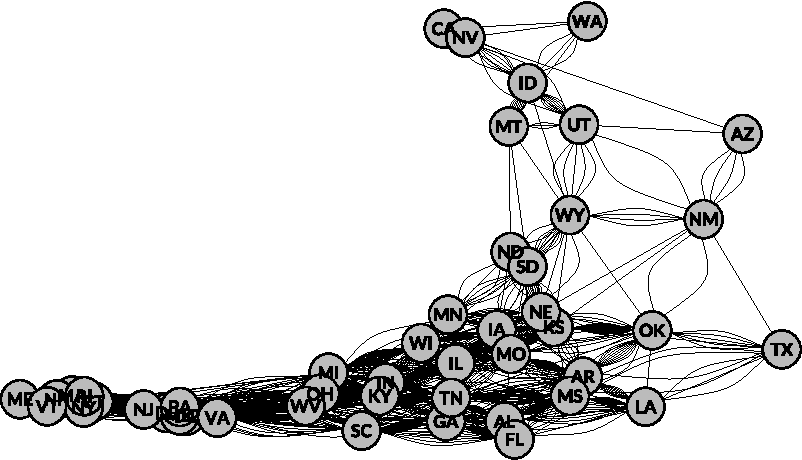
\includegraphics[width=1\linewidth]{assignment3_files/figure-latex/plot_graph-1} \end{center}

\begin{Shaded}
\begin{Highlighting}[]
\FunctionTok{heatmap}\NormalTok{(cigk, }\AttributeTok{Rowv =} \ConstantTok{NA}\NormalTok{, }\AttributeTok{Colv =} \StringTok{"Rowv"}\NormalTok{)}
\end{Highlighting}
\end{Shaded}

\begin{center}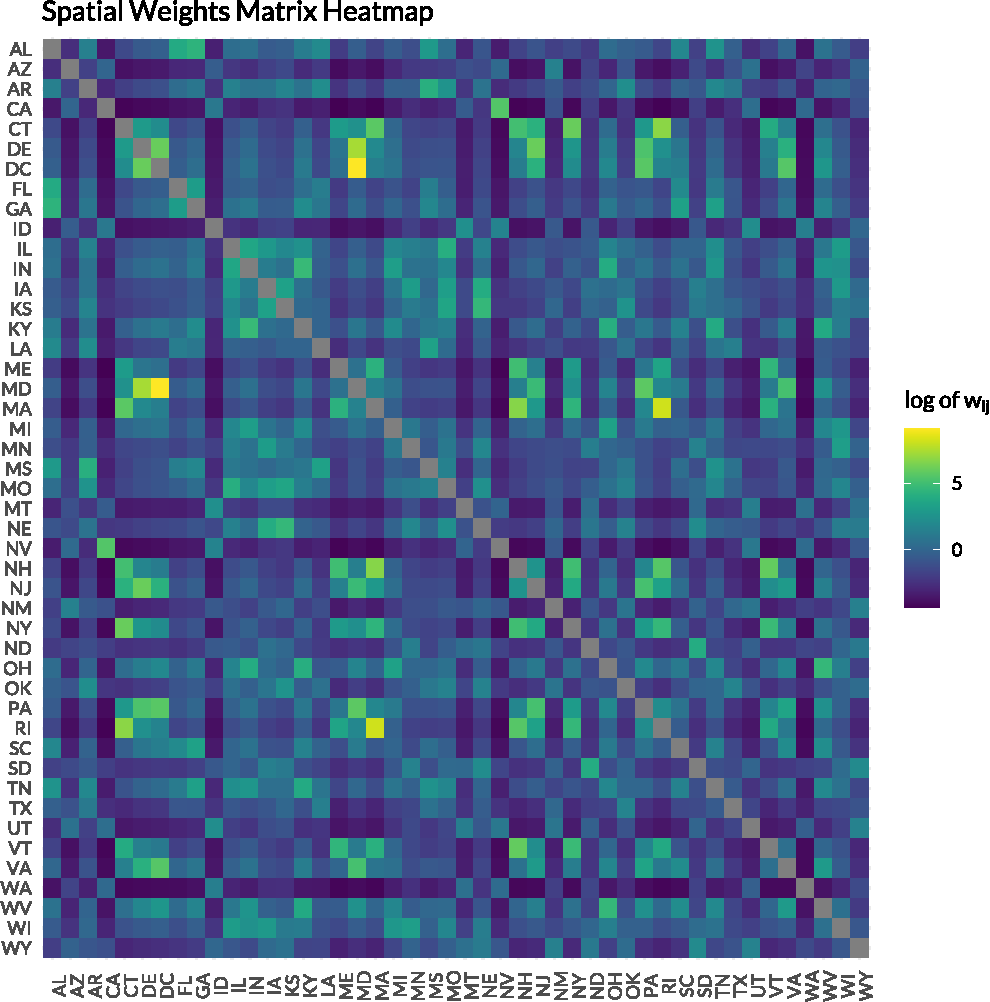
\includegraphics[width=0.6\linewidth]{assignment3_files/figure-latex/plot_heatmap-1} \end{center}

\begin{Shaded}
\begin{Highlighting}[]
\FunctionTok{rowSums}\NormalTok{(cigk) }\SpecialCharTok{\%\textgreater{}\%}
    \FunctionTok{sort}\NormalTok{(}\AttributeTok{decreasing =} \ConstantTok{TRUE}\NormalTok{) }\SpecialCharTok{\%\textgreater{}\%}
\NormalTok{    knitr}\SpecialCharTok{::}\FunctionTok{kable}\NormalTok{(}\AttributeTok{col.names =} \StringTok{"Row Sum"}\NormalTok{)}
\end{Highlighting}
\end{Shaded}

\begin{longtable}[]{@{}lr@{}}
\toprule\noalign{}
& Row Sum \\
\midrule\noalign{}
\endhead
\bottomrule\noalign{}
\endlastfoot
MD & 11026.67198 \\
DC & 9945.46534 \\
RI & 4756.35048 \\
MA & 4728.87454 \\
DE & 2663.12139 \\
CT & 1913.64955 \\
NH & 1878.45853 \\
PA & 1082.00099 \\
NJ & 983.52610 \\
NY & 968.47870 \\
VT & 746.96390 \\
VA & 615.20596 \\
ME & 386.75814 \\
KY & 333.66481 \\
OH & 308.21679 \\
IN & 303.99804 \\
WV & 271.93286 \\
NV & 253.46415 \\
CA & 248.41830 \\
KS & 215.91668 \\
NE & 209.03832 \\
IL & 207.81238 \\
GA & 201.84045 \\
AL & 193.97210 \\
MO & 191.43001 \\
IA & 185.93943 \\
TN & 176.79008 \\
MS & 160.89378 \\
AR & 140.08363 \\
WI & 127.73114 \\
MI & 123.99357 \\
SC & 100.11099 \\
FL & 98.10254 \\
SD & 90.44541 \\
MN & 85.93133 \\
ND & 71.63010 \\
LA & 70.08663 \\
OK & 60.44297 \\
WY & 38.15529 \\
ID & 35.44483 \\
UT & 32.25951 \\
TX & 25.43502 \\
MT & 25.15952 \\
NM & 24.47703 \\
AZ & 14.19491 \\
WA & 10.75984 \\
\end{longtable}

\begin{longtable}[]{@{}lr@{}}
\toprule\noalign{}
& Eigenvector Centrality \\
\midrule\noalign{}
\endhead
\bottomrule\noalign{}
\endlastfoot
MD & 1.0000000 \\
DC & 0.9871728 \\
DE & 0.2112788 \\
PA & 0.0682453 \\
VA & 0.0486044 \\
NJ & 0.0310696 \\
CT & 0.0033553 \\
WV & 0.0030710 \\
RI & 0.0028691 \\
NY & 0.0025882 \\
MA & 0.0023642 \\
OH & 0.0013980 \\
NH & 0.0013860 \\
VT & 0.0008475 \\
SC & 0.0007672 \\
KY & 0.0006332 \\
IN & 0.0003951 \\
MI & 0.0003824 \\
ME & 0.0003685 \\
GA & 0.0002656 \\
TN & 0.0002394 \\
AL & 0.0000095 \\
IL & 0.0000043 \\
WI & 0.0000021 \\
FL & 0.0000017 \\
MO & 0.0000013 \\
MS & 0.0000012 \\
IA & 0.0000005 \\
AR & 0.0000005 \\
MN & 0.0000003 \\
KS & 0.0000002 \\
LA & 0.0000001 \\
NE & 0.0000001 \\
OK & 0.0000000 \\
SD & 0.0000000 \\
TX & 0.0000000 \\
ND & 0.0000000 \\
WY & 0.0000000 \\
NM & 0.0000000 \\
MT & 0.0000000 \\
UT & 0.0000000 \\
AZ & 0.0000000 \\
ID & 0.0000000 \\
NV & 0.0000000 \\
CA & 0.0000000 \\
WA & 0.0000000 \\
\end{longtable}

\newpage

\hypertarget{task-b}{%
\section{Task B}\label{task-b}}

\hypertarget{task-b.1---unit-of-observation}{%
\subsection{Task B.1 - Unit of
Observation}\label{task-b.1---unit-of-observation}}

Describe the unit of observation: * subnational ``cells''
--\textgreater{} grid squares * used to conduct a geographically
disaggregated analysis of civil conflict and weather shocks

What are their areas? * cells have dimensions of 110 km by 110 km
(square)

Why and to which (relative) extent do they differ? * spatial resolution?

\hypertarget{task-b.2---un-normalized-weights-matrix}{%
\subsection{Task B.2 - Un-normalized weights
matrix}\label{task-b.2---un-normalized-weights-matrix}}

\newpage

\printbibliography

\end{document}
